\documentclass[xcolor=dvipsnames,table]{beamer}

\usepackage{latexsym}
\usepackage[utf8]{inputenc}
\usepackage[brazil]{babel}
\usepackage{amssymb}
\usepackage{amsmath}
\usepackage{stmaryrd}
\usepackage{fancybox}
\usepackage{datetime}
\usepackage[T1]{fontenc}
\usepackage{graphicx}
\usepackage{graphics}
\usepackage{url}
\usepackage{algorithmic}
\usepackage{algorithm}
\usepackage{acronym}
\usepackage{array}

\newtheorem{definicao}{Definio}
\newcommand{\tab}{\hspace*{2em}}

\mode<presentation>
{
  \definecolor{colortexto}{RGB}{0,0,0}
 
  \setbeamertemplate{background canvas}[vertical shading][ bottom=white!10,top=white!10]
  \setbeamercolor{normal text}{fg=colortexto} 

  \usetheme{Warsaw}
}

\title{Conjuntos estáveis} 

\author{
  Esdras Lins Bispo Jr. \\ \url{bispojr@ufg.br}
  } 
 \institute{
  Teoria de Grafos \\Bacharelado em Ciência da Computação}
\date{\textbf{26 de julho de 2016} }

\logo{
\includegraphics[width=1cm]{images/ufgJataiLogo.png}}

\begin{document}

	\begin{frame}
		\titlepage
	\end{frame}

	\AtBeginSection{
		\begin{frame}{Sumário}%[allowframebreaks]{Sumário}
    		\tableofcontents[currentsection]
    		%\tableofcontents[currentsection, hideothersubsections]
		\end{frame}
	}

	\begin{frame}{Plano de Aula}
		\tableofcontents
		%\tableofcontents[hideallsubsections]
	\end{frame}
	
	\section{Pensamento}
	\begin{frame}{Pensamento}
  		\begin{center}
    		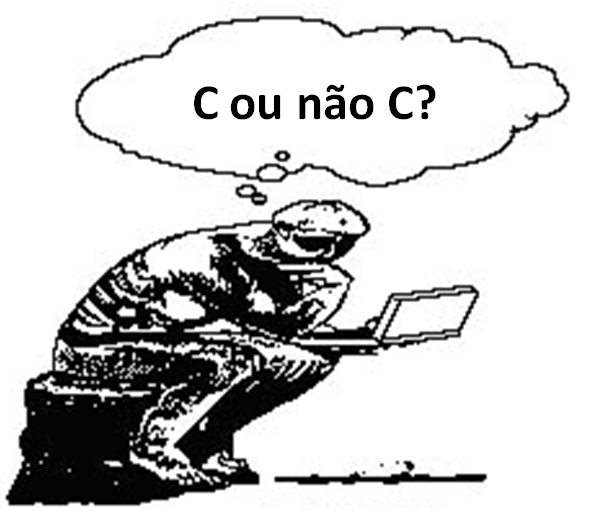
\includegraphics[width=7cm]{images/pensamento.png}
  		\end{center}
	\end{frame}
	
	\begin{frame}{Pensamento}
		\begin{columns}
			\column{.4\textwidth}  		
		  		\begin{center}
		    		
\includegraphics[height=.5\textheight]{images/desconhecido.jpg}
		  		\end{center}
			\column{.6\textwidth}  		
				\begin{block}{Frase}
					\begin{center}
						{\large Quando o machado entrou na floresta, as árvores disseram: \\- O cabo é dos nossos!!}
					\end{center}
				\end{block}		  		
		  		\begin{block}{Quem?}
		  			\begin{center}
						{\bf Provérbio Turco}
					\end{center}
				\end{block}
		\end{columns}
	\end{frame}
    
	\begin{frame}{Bônus (0,5 pt)}
		\begin{block}{Desafio}
			\begin{itemize}
				\item {E 2.20} 
                \item Candidaturas agora; 
                \item Apresentação e resposta por escrito $\rightarrow$ \\Terça (02 de agosto, 15h30); 
                \item 20 minutos de apresentação.
			\end{itemize}
		\end{block}
        \begin{block}{Referência}
			FEOFILOFF, P. {\bf Exercícios de Teoria dos Grafos}, \\
			BCC, IME-USP, 2012. 
		\end{block}	
	\end{frame}    
    
    \section{Revisão}
	
	
	\subsection{Isomorfismo}
	\begin{frame}{Isomorfismo}
		\begin{block}{Definição}
			Um {\bf isomorfismo} entre dois grafos $G$ e $H$ é uma bijeção $f$ de $V(G)$ em $V(H)$ tal que dois vértices $v$ e $w$ são adjacentes em $G$ se e somente se $f(v)$ e $f(w)$ são adjacentes em $H$. Dois grafos são {\bf isomorfos} se existe um isomorfismo entre eles.
		\end{block}
		\begin{block}{Problema}
			Dado dois grafos $G$ e $H$, verificar se existe um isomorfismo entre eles.
		\end{block}
		\begin{block}{Solução}
			Basta examinar todas as bijeções de $V(G)$ e $V(H)$. Se cada um dos grafos tem $n$ vértices, esse algoritmo consome tempo proporcional a $n!$.
		\end{block}
	\end{frame}
	
	\begin{frame}{Isomorfismo}
		\begin{center}
			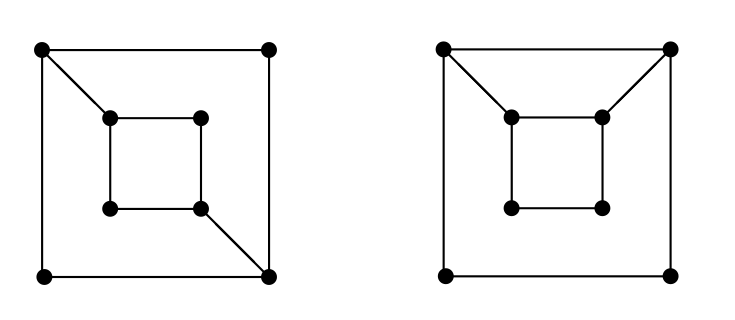
\includegraphics[width=8cm]{images/isomorfismo01.png}
		\end{center}
	\end{frame}
	
	\begin{frame}{Isomorfismo}
		\begin{center}
			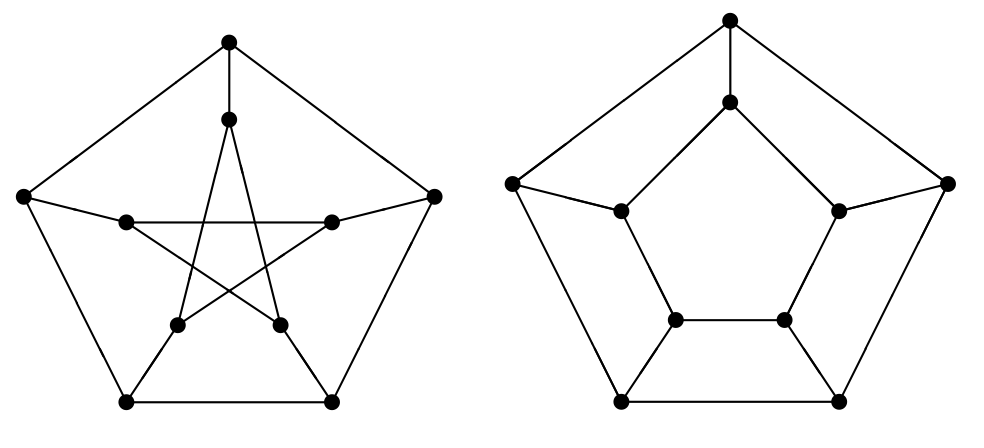
\includegraphics[width=8cm]{images/isomorfismo02.png}
		\end{center}
	\end{frame}
	
	\begin{frame}{Isomorfismo}
		\begin{center}
			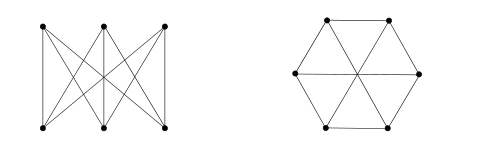
\includegraphics[width=10cm]{images/isomorfismo03.png}
		\end{center}
	\end{frame}
	
	\begin{frame}{Isomorfismo}
		\begin{block}{Corolário 01}
			Se $G$ e $H$ são isomorfos, então $|V(G)| = |V(H)|$.
		\end{block}
		\begin{block}{Corolário 02}
			Se $G$ e $H$ são isomorfos, então $|A(G)| = |A(H)|$.
		\end{block}
		\begin{block}{Corolário 03}
			Se $G$ e $H$ são isomorfos, então $\delta(G) = \delta(H)$ e $\Delta(G) = \Delta(H)$.
		\end{block}
	\end{frame}
	
	\section{Conjuntos Estáveis}
	\begin{frame}{Conjuntos Estáveis}
		\begin{block}{Definição}
			Um conjunto $X$ de vértices de um grafo é {\bf estável} ({\it = stable = independent}) se seus elementos são dois a dois não adjacentes.
		\end{block} \pause
		\begin{block}{Corolário 1}
			$X$ é estável se nenhuma aresta do grafo tem ambas as pontas em $X$.
		\end{block} \pause
		\begin{block}{Corolário 2}
			$X$ é estável se $G[X] = \overline{K_n}$.
		\end{block} 
	\end{frame}
	
	\begin{frame}{Conjuntos Estáveis}
		\begin{block}{Problema do Conjunto Estável Máximo}
			Encontrar um conjunto estável máximo num grafo dado.
		\end{block} \pause
		\begin{block}{Variação do Problema}
			Dado um grafo e um número natural $k$, encontrar um conjunto estável com $k$ ou mais vértices.
		\end{block} \pause
		\begin{block}{Tamanho do conjunto estável máximo de um grafo $G$}
			\begin{center}
				$\alpha (G)$
			\end{center} \pause
			em inglês chama-se {\bf stability number} ou {\bf indepedence number}. \pause Poderíamos chamar de {\bf índice de estabilidade}.
		\end{block}
	\end{frame}
	
	\begin{frame}
		\titlepage
	\end{frame}
	
\end{document}